%%%%%%%
% This chapter is all about setting the vision for the work, and listing contributions 
%%%%%%%
\chapter{Introduction}
\label{chap:intro}

\begin{center}
    \begin{minipage}{0.7\textwidth}
      \begin{small}
       It is a wholesome and necessary thing for us to turn again to the earth and in the contemplation of her beauties to know the sense of wonder and humility.\\ \emph{Rachel Carson}
      \end{small}
    \end{minipage}
    \vspace{0.5cm}
\end{center}


% Our pale blue dot\footnote{a term coined by Carl Sagan reflecting on a photo Voyager I snapped of Earth on it's trek out of the Solar System} is home to broad classes of flora and fauna.
% That blue comes from the hue of the planet's liquid water oceans, which cover the majority of the planet's surface.

The environmental sciences are the multidisciplinary, academic studies which aim to understand the Earth and its processes.
\emph{In situ} observational studies, or \emph{expeditions}, serve as the foundation on which scientific discovery and model development are predicated in these fields.
With improvements in technology, expeditions have been conducted in the deepest trenches of the ocean to the uppermost atmosphere.
Improved reach, in addition to improved observational quality, density, and availability has made it increasingly clear how inextricably entwined Earth's regulatory processes are, and how crucial a role the ocean plays in these processes.
Covering 70\% of the Earth's surface, the ocean is the largest biosphere on the planet, home to a staggering number of unique microorganisms up to the largest creatures on Earth, ultimately encompassing over 90\% of the habitable volume on Earth\autocite{cario2019exploring,purkis2022remote}.
The plant life supported by the ocean and ocean-coast interfaces are estimated to absorb 50\% of all excess carbon dioxide emissions produced by anthropogenic sources, acting as a buffer to global heating\autocite{hori2019blue}.
Culturally, the ocean is also entwined with our sense of humanity and development of society---island and coastal habitats supported the earliest hominids\autocite{erlandson2006oceans}, traveling the ocean has shaped trade, conquest, and tradition\autocite{pearson2003indian,chaudhuri1985trade,firth2019understanding,nunn2003nature}, and the ocean inspires creativity, recreation, and curiosity.
Despite the centrality of the ocean to existence (and continued existence) as we know it on Earth, there is yet so much that has yet to be discovered.

In the last decade, significant effort has been put to finely mapping the seafloor\footnote{e.g., through Seabed 2030~\autocite{mayer2018nippon}, among other initiatives}, and as of mid-2022 nearly a quarter of the seafloor has been mapped bathymetrically in high resolution (compared to about 6\% in 2017)\footnote{As reported by Seabed 2030 at \url{https://seabed2030.org/mapping-progress}.}. 
High resolution maps allow us to better understand continental drift and crustal processes, the distribution of natural resources, and the ecosystems which ocean structures can support.
Unlike terrestrial environments, which can be largely observed remotely (either by aircraft, or more commonly now, satellite), the ocean, especially the deep ocean, cannot be globally observed due to the conductive properties of water and it's tendency to absorb many forms of light and radio energy.
Mapping the seafloor requires physically going to sea.
The mapping revolution of the ocean is enabled thanks in part\footnote{In other part, it has been enabled by an increased economic and political commitment to the ocean, it's strategic value, and the resources contained within it.} to improved acoustic technology and processing tools, which allow shipboard acoustic sounders to collect high resolution ``imagery'' while traversing on the surface ocean.

Bathymetry is one piece of the giant puzzle that is the ocean; another piece seeing contemporary scrutiny is geochemistry of the deep ocean.
Geochemistry, the study of Earth and other planetary geological systems through chemical principles, enables us to understand the processes which create and sustain the structures that bathymetric maps reveal, and tell us more about local ecosystems and their nutrient and energetic budgets. 
Geochemical measurements may range from studying the composition of rock samples from the seafloor, to \emph{in situ} observations of dissolved gases in a hydrothermal plume.
Modern interests in seafloor mining to remove materials from the deep ocean\autocite{thompson2018seabed}, and deep ocean carbon sequestration to inject the ocean with excess materials\autocite{teng2018long}, stand to directly impact the balance of the deep biogeosphere, with implications that have yet to be well understood (or agreed upon) by science\autocite{smith2020deep,seibel2001potential,fleeger2010response,sharma2015environmental,childs2020extraction,van2011tighten}.
Unlike acoustic surveys, which even though highly localized can be performed from a ship hundreds or thousands of meters above the seabed, geochemical surveys must truly be conducted \emph{in situ} with instruments physically sent to the deep ocean to collect continuous measurements, or physical bottle samples of water or rock specimens retrieved for \emph{ex situ} analysis.
There is an ongoing paradigm shift in ocean technology to better enable geochemical studies of the deep ocean: development of novel \emph{in situ} sensors, creation of more depth-capable instruments, and adoption of autonomous technologies for sample collection or expedition planning. 

Intelligent autonomous technologies are any systems which can automatically process and analyze a data product, and formulate evidence-based decisions which they may then act upon.
These systems may be \emph{embodied}, like robotic vehicles, or simply algorithmic.
A science party member at sea can be viewed as an intelligent autonomous agent for an expedition: the scientist will be collecting and processing data throughout the voyage, using that data to coordinate with other science party members to design activities, and managing the deployment of various sensors and platforms.
Good algorithmic or robotic contributions relieve the burden of data processing and decision-making on the science party to make their time, the expedition time, and the resources aboard a vessel more effective.
For marine geochemical surveys, one of the key challenges for the science party to grapple with is understanding \emph{spatiotemporal distributions}, which are nearly ubiquitous in water column studies.
A spatiotemporal distribution is a phenomenon that evolves in space and time; in the deep sea, these may take the form of hydrothermal plumes, hydrate dissolution, sediment transport, or water mass mixing.

\emph{Perceiving} a spatiotemporal distribution from sparse \emph{in situ} measurements; \emph{predicting} the evolution of the distribution into future expedition dates or sites; and \emph{planning} where and when to take samples of the phenomenon for further inspection, are key challenges for any autonomous agent.
This thesis presents several algorithmic and operational strategies for addressing these challenges for deep ocean geochemical surveys, with a particular contextual focus on charting the spatiotemporal structure of hydrothermal plumes.
The algorithmic contributions of this thesis are motivated by tools used in the discipline of robotics to enable \emph{planning under uncertainty}; a technique for decision-making with incomplete information about a target environment or task.
In planning under uncertainty architectures there are many design choices available to an engineer---how data is processed, how the data is used to construct a \emph{belief} about the environment or task, and how that belief is leveraged to pick actions to take.
Field and scientific contexts provide constraints and requirements that shape the feasible set of design choices that can be made, sometimes requiring creativity outside the pale in theoretical research.
A core tenant of the research presented here is a field roboticist has a special responsibility to ensure that the solutions that are engineered accomplish the science that they were designed for.
In line with this, scientific results which enhance understanding about deep sea hydrothermal plumes are found throughout this thesis, in balance with formulation and assessment of autonomous technologies.

In the rest of this chapter, an overview of deep hydrothermalism and geochemical field operations is provided, in addition to a summary of specific algorithmic challenges and the techniques employed in this thesis to overcome them.
A brief contribution statement concludes the chapter.

% This research spans practical to theoretical challenges and considerations, and was performed in close collaboration with scientists and engineers in fields including oceanography and geochemistry, computational statistics, robotics, and data science.
% Chief among the challenges addressed in this research is the problem of uncovering the underlying dynamics of a spatiotemporal distribution.


%%%%%%%%%%%%%%%%%%%%%%%%%%%%%%%%%%
% Hydrothermal Plume Charting
%%%%%%%%%%%%%%%%%%%%%%%%%%%%%%%%%%
\section{Hydrothermalism in the Deep Ocean}
\label{sec:charting-plumes}
The deep ocean is considered to be any part of the ocean at least \SI{200}{\meter} below sea-level\footnote{Some literature more specifically claims the deep ocean to be at least \SI{1000}{\meter} below the surface. I will use the \SI{200}{\meter} definition, unless otherwise stated.}.
Volumetrically, the deep ocean is \emph{most} of the ocean, and life has been discovered at every depth, including the Challenger Deep, the deepest point on Earth at nearly \SI{110000}{\meter}\autocite{cario2019exploring}\footnote{Interestingly, the average depth of the ocean is approximately \SI{3800}{\meter}; above sea-level, the average height of land is \SI{840}{\meter}.}.
A persistent adage in the ocean sciences is that more is known about the surface of other worlds than about our own deep ocean.
This is poignantly illustrated with the first observation of hydrothermal vents in 1977 at the Galápagos Rift~\autocite{corliss1979submarine}, 8 years after humans walked on the moon for the first time.

Since 1977, hundreds of vents have been discovered and studied around the world\autocite{beaulieu2013authoritative}, and subject of increasingly urgent conversations about characterizing the deep ocean.
Seafloor venting sites, energized by magmatic sources, release fluids between 20-\SI{400}{\celsius} (background deep ocean temperatures are approximately \SI{2}{\celsius}) and imbued with minerals, metals, dissolved gases, and other compounds~\autocite{jannasch1985geomicrobiology, martin2008hydrothermal}.
These warm, nutrient-pumping sites in the deep ocean have created oases for unique micro- and macro-fauna~\autocite{corliss1979submarine}, and the venting fluids, called plumes, can deposit minerals and metals over kilometer (basin) scales\autocite{scholz2019shelf,resing2015basin,le2019hydrothermal}.
Detection and characterization of seafloor hydrothermal venting are critical for understanding fundamental interactions between the deep ocean, its underlying basaltic crust, the deep biosphere, and (bio)geochemical fluxes.

To study hydrothermalism in the deep ocean, rosettes\footnote{Rosettes are often a metal cage with instrumentation and bottles that is attached to a ship via a cable; it can be raised and lowered in the water column with a shipboard winch.}, remotely-operated vehicles (ROVs), human occupied vehicles (HOVs), and autonomous underwater vehicles (AUVs) all equipped with specialized \emph{in situ} instrumentation and often bottles for water sampling, are available.
ROVs and HOVs have enabled detailed study of venting chimneys and diffusive venting fields on the seafloor, literally ``putting eyes'' on the structures and physically interacting with them.
To study plumes generated by vents, AUVs and rosettes can be used to examine the water column.
However, using these technologies to produce detailed studies of plumes is more challenging than studying a vent; plume signal is naturally variable, turbulent, and ephemeral and navigating in the water column is a logistical challenge due to lack of physical features by which to navigate or localize. 
Thus, many detections of a plume tend to be serendipitous in practice.

To leverage these detections, laboratory experiments to model how plumes are expected to manifest in the water column have served a critical role in converting field observations to statements about energetic characteristics, nutrient transport, and overall impact in a basin.
Among the most widely used models that describe hydrothermal plumes are the Morton, Taylor, and Turner (MTT) model for buoyant plumes derived in the 1950s~\autocite{morton1956turbulent}, and the re-derivation specifically for hydrothermal plumes in the late 1980s by Speer and Rona~\autocite{speer1989model}.
These idealized (time-averaged) models describe a roughly two part plume structure composed of a buoyant stem and a neutrally-buoyant layer. 
The buoyant stem is a spatially small expression that describes the fluid that rapidly rises from an originating vent orifice, driven by buoyant forces that result in the difference in density between the warm venting fluid and the ambient seawater.
The neutrally-buoyant\footnote{This can be equivalently styled as non-buoyant.} layer describes the spatially large spread of vent-derived fluids along the isopycnal of equal density with the ambient seawater (\cref{fig:intro_summary}\footnote{Readers are additionally referred to~\autocite{yoerger2007autonomous} for an illustrative description and figure.}). 
State-of-the-art hydrothermal plume models incorporate time-varying Navier-Stokes models and more complicated fluid structures\footnote{e.g.,~\autocite{lavelle2013turbulent,xu2012deep}}.
Mathematically, these models describe what has been practically well-understood in observational studies: the spatiotemporal distribution of plumes is instantaneously complicated and on small scales (meters, minutes) driven by compounding, chaotic factors that are difficult to calibrate.



\begin{figure}[h!]
  \centering
  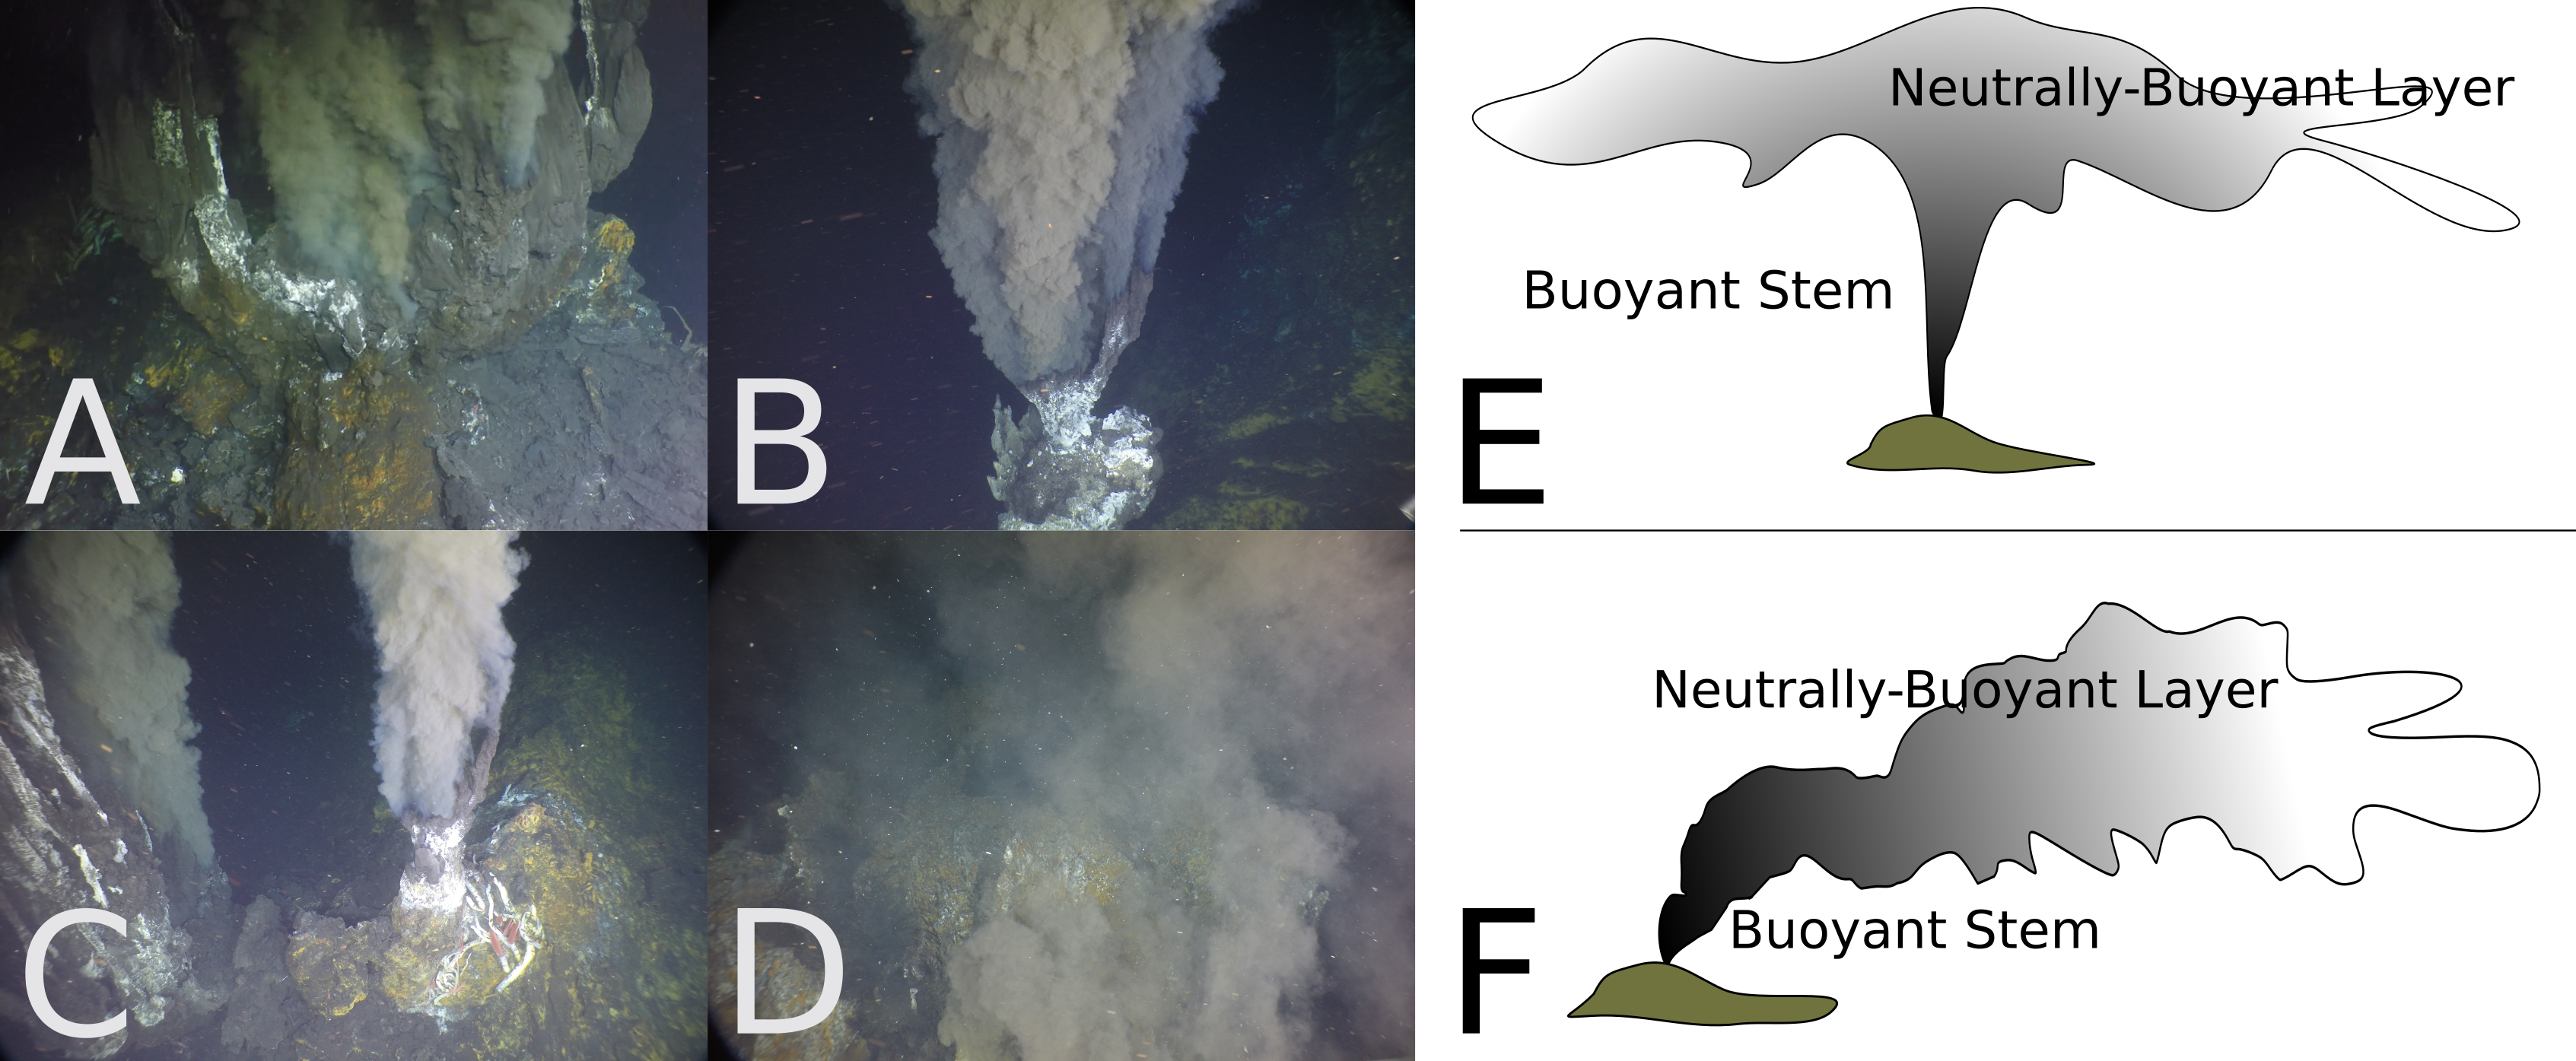
\includegraphics[width=1\columnwidth]{figures/intro_hydro.png}
  \caption[Images of hydrothermal vents and illustrative plume structures.]{\textbf{Images of hydrothermal vents and illustrative plume structures.} Images A-D are different hydrothermal vents observed by remotely operated vehicle (ROV) \emph{JASON} at Guaymas Basin, Gulf of California (Mexico) in November 2021 during a science expedition. A and B show how vents in the basin were formed of many small orifices, creating a complicated chimney structure producing large, turbid plumes. C shows two co-located vent clusters. D is an image of a more diffusive turbid plume. Panels E-F are illustrative examples of plume structures, without crossflow (E) and with crossflow (F). The buoyant stem tends to be a relatively small, coherent structure that rises approximately 100-\SI{300}{\meter} in a water column (depending on the character of the plume fluid and background seawater). The neutrally-buoyant layer can be spatially large (on the order of kilometers), but tends to be more diffuse and is found at a height of equal density with the ambient seawater. Crossflow impacts the ultimate rise height of a plume, and the amount of ambient seawater that is entrained (mixed) as the plume evolves.}
  \label{fig:intro_hydro}
\end{figure}


Field measurements are used to set the initial conditions or parameters of a numerical model, which is then used in turn to make claims about characteristics of a plume.
This is widely known as solving an \emph{inverse problem}; using observations to find an explanatory set of variables (e.g., initial conditions, numerical parameters).
One of the key challenges of solving an inverse problem with observations in the sciences is that the problem is mathematically ill-posed; that is, it is difficult to find the correct, unique solution due to noise in the observations and the time/space that those observations were taken.
For instance, observations along or near the exact centerline of a plume may be significantly more informative about the vent characteristics\autocite{bangian2022solution} than samples randomly collected throughout a plume structure\autocite{baker1998rise}.
But given that most field measurements are serendipitous, solving the inverse problem to an acceptable level of accuracy requires grappling with \emph{uncertainty}\footnote{Both epistemic and aleatoric. Aleatoric uncertainty in this case comes from the chaotic nature of spatiotemporal distributions (for instance, turbulent flows). Epistemic uncertainty is definitional, as we have uncertainty of the model and noisy observations.}.
Probabilistic representations or analytical models of uncertainty have been used in plume studies to help place confidence intervals over found solutions\autocite{bemis1993geothermal,sohn2019observations}.
In classical studies, uncertainty is computed following an expedition and after all data is available.
In this thesis, an algorithmic extension to the classical uncertainty formalism is extended to enable practical-time inference of plume characteristics while at sea.
By computing a notion of uncertainty while at sea, strategic changes to the science activities and instrument deployments can be undertaken to target collection of more informative samples.



% over the underlying dynamics of a target environment due to the extreme partial observability of point \emph{in situ} measurements in a continuous three-dimensional volume over time influenced by complicated spatiotemporal dynamics of water mixing, tidal advection, and chaotic turbulence.
% The notion of uncertainty has implications for solving both the \emph{inverse} and \emph{forward} problem inherently posed in hydrothermal plume charting.
% Discovering the underlying model from a set of data, the inverse problem, is known to be ill-posed in spatiotemporal systems CITE, suggesting that the information content of every sample has an outsized effect on the accuracy of recovered dynamics.
% With a known dynamics model, forward simulating a model with uncertainty placed over initial conditions or descriptive parameters requires propagating that uncertainty forward.
% In time-dependent models, even modest amounts of uncertainty can accumulate quickly over short horizons CITE, yielding essentially uninformative predictive state estimates for planning.
% A principled treatment of uncertainty, particularly the identification of \emph{useful} uncertainty for planning, is necessary. 
% WORDS ON HOW PEOPLE HAVE THOUGHT ABOUT UNCERTAINTY IN HYDROTHERMAL SYSTEMS


% Questions related to mineral and metal deposition from plumes highlight the acute scientific need to better study not just hydrothermal vents themselves, but the plume structures that are produced by them which are the primary drivers of nutrient injection in the deep ocean biosphere.
% Scientific studies that benefit from directly charting the spatiotemporal structure of a plume include those which characterize the transport and deposition of particulates, the distribution and transport of biological materials (including microbes) in the deep ocean, and field-based statistical modeling of turbulent water mass mixing.


%%%%%%%%%%%%%%%%%%%%%%%%
% Autonomy Challenges
%%%%%%%%%%%%%%%%%%%%%%%%
\section{Challenges for Intelligent Autonomy}
For geochemical studies in the water column, AUVs are uniquely well-positioned to advance long-term monitoring of and exploration in mesoscale\footnote{Tens of meters to several kilometers} deep ocean environments during \emph{in situ} expeditions.
Autonomy for a robotic system can fall on an ``agency'' spectrum: a robot with full agency can make adjustments to its own behavior; a robot with no agency can execute a pre-determined set of tasks without supervision, but cannot change the tasks while performing.
Increasingly, AUVs are being developed for deep sea research\autocite{kaiser2016design,yuh2000design,okamoto2019visual,maki2014auv}, but their autonomous capabilities are typically limited to executing predetermined hand-designed trajectories such as uniform coverage lawnmowing patterns~\autocite{camilli2010tracking}, falling into the category of robots without agency.
This restriction is often applied in order for trajectories to be rigorously checked by engineering teams prior to execution as an operational policy of risk reduction, and for ease of supervision during execution.

Operating without agency necessarily restricts the class of phenomena that can be effectively studied by expeditionary robots used in the science fleet today.
Using non-adaptive surveying strategies, spatiotemporal distributions can be severely under-sampled or missed completely\autocite{flaspohler2019information, preston2019adaptive}.
This can be mitigated when the underlying model of the spatiotemporal dynamics is known, but for reasons explained in the previous section, in field settings a dynamics model must be estimated from data because the environmental condition is initially unknown (\cref{fig:intro_traj}).
This estimation process is challenging, as data that can be collected in real field trials tends to be noisy and extremely \emph{partially observable}---that is, the observations are only at point locations in time and space, and may be indirect measurements of a desired field of interest. 
Consequently, classical data-driven modeling techniques used in robotics to describe the environment in which a robot finds itself, such as Guassian Processes\autocite{Rasmussen2004}, neural networks\autocite{cohn1994neural,wang2017predrnn}, or particle representations\autocite{Silver2010}, would require many observations to generalize to a useful model for planning; a luxury that, in the field, is typically not afforded due to limited opportunities for deployments and finite expedition timelines.


\begin{figure}[h!]
  \centering
  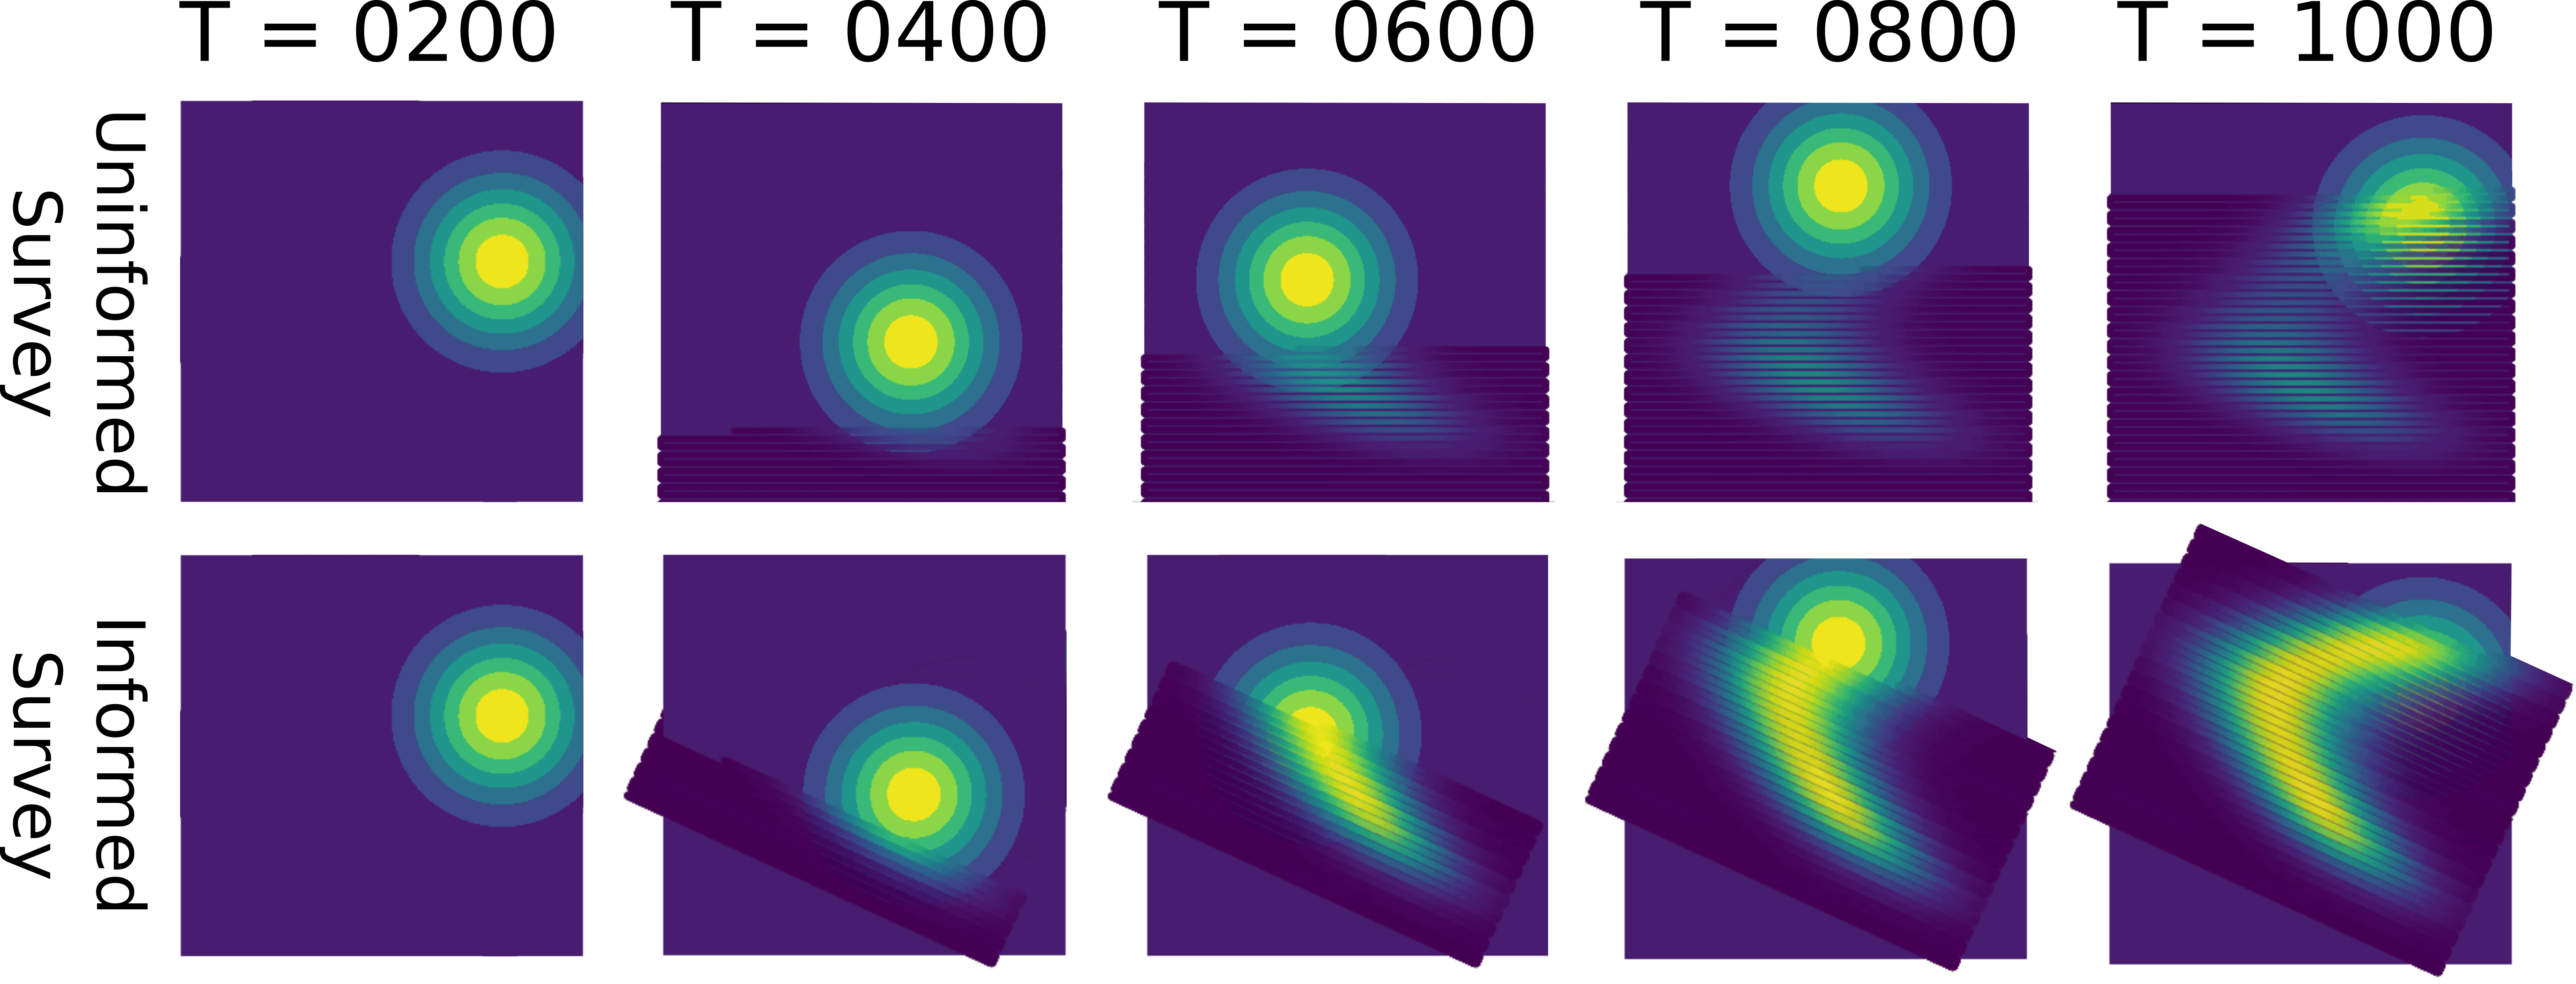
\includegraphics[width=1\columnwidth]{figures/intro_lawn.png}
  \caption[Comparison of informed and uninformed survey of spatiotemporal distribution.]{\textbf{Illustrative comparison of an informed and uninformed survey of a spatiotemporal distribution.} Several snapshots of an illustrative ``bullseye'' world are provided, in which two lawnmower trajectories are planned. At each time snapshot, the collected observations by the two surveys are plotted on top of the true underlying phenomenon. In the top row, an uninformed lawnmower starts in the bottom right corner of the world and travels upward.  Most samples collected are at the fringes of the bullseye distribution. In contrast, the bottom row shows a lawnmower with all of the same characteristics (resolution, height, width) with an adjusted orientation, informed by the knowledge of the underlying bullseye dynamic. This survey collects a significant number of samples at the center of the bullseye and effectively tracks the phenomenon throughout the duration of the simulated mission.}
  \label{fig:intro_traj}
\end{figure}

Access to numerical models of plume dynamics stands to significantly relieve the burden on data alone to recover a descriptive model of the target environment during an expedition.
Scientific machine learning (SML), an emerging subfield of machine learning, has shown that leveraging numerical scientific models of physical principles within classically data-driven frameworks\autocite{raissi2019physics, sapsis2009dynamically, mohan2019compressed,raissi2018numerical,kulkarni2019advection, brunton2016discovering,jiahao2021knowledge} can improve the data efficiency of a learner and the overall quality of the model that is uncovered.
To extend SML algorithmic theory to field settings, in which computational time is limited and field observations are corrupted with noise (and significantly partially observable), requires careful selection of both the underlying numerical model and the learning framework that wraps it.
Foundational principles (e.g., conservation of mass, non-divergence) and idealized, time averaged models (e.g., MTT\autocite{morton1956turbulent}), provide an informative basis on which to learn that describes the ``shape'' of a plume distribution, but abstracts the details away for tractable computation.
Notionally, the idea of using a simplified basis on which to perform inference relates closely with reduced order modeling techniques in dynamical control theory and computational sciences\autocite{lucia2004reduced,burkardt2006pod,salam2019adaptive} or latent space discovery in machine learning\autocite{voynov2020unsupervised,lu2020extracting}.
In these works, the aim is to uncover the smallest set of basis vectors/functions to describe a phenomenon to a desired level of accuracy.
Instead of discovering these spaces via data however (which would require too many samples, full-state observations, or an infeasible number of AUV deployments), the ``latent space'' is directly set by the initial conditions and parameters of a numerical model, and it's relationship to the observational space is the model itself.
The inference framework that then sits on top of that model can ``absorb'' uncertainty due to the mismatch between the resolution of the model and the instantaneous measurements that are collected, can be used to describe unmodeled characteristics (i.e., act as a probabilistic closure model), or simply extend the representation of the model to enable computation of information-theoretic measures that can assist with decision-making.
% As some in robotics may say, however, there is no free lunch.
% The use of physically-informed structure trades sample efficiency for increased computational cost at deployment time (in comparison to purely data-driven techniques).
% However, this trade-off can be tuned for the underlying models available, the sampling task at hand, and the operational logistics during field opportunities.


In practice, embedding scientific knowledge into probabilistic models (i.e., belief representations) for planning requires additional algorithmic infrastructure that (1) casts AUV observations into a space that aligns with the solution of the numerical model, and (2) can design operationally satisfactory sampling trajectories that leverage belief effectively.
Scientific observations are typically taken by heterogeneous sensors with different operating principles.
In the case of hydrothermal plumes, there is no ``plume-detector'' available for an AUV, instead measurements from a scientific sensor suite must be collectively examined.
While some numerical models provide projections of plumes that include observable quantities\autocite{speer1989model} (e.g., temperature, salinity), many more instead provide a generic ``tracer'' distribution that does not neatly map to sensors that are available on an AUV.
Thus, to fingerprint a plume from data requires characterizing the potentially complicated interrelationships between sensor measurements\autocite{jakuba2007stochastic}.
Science experts are particularly good at this task, as they often have years of intuition for the data, experience with specific scientific instruments, and domain knowledge of how plumes have manifested in other studies.
In this thesis, tools that assist science experts with identifying hydrothermalism from long AUV surveys (which can be tens of thousands of point observations), and a fully automatic detector informed by science expertise, are presented.
The latter is subsequently used as the observation model for the physically-informed belief representation to assist in downstream planning tasks.

% While it is unreasonable to assume that a roboticist become a domain expert in a particular scientific field in order to plan useful trajectories, familiarity with the forms, limitations, and working principles of critical science sensing infrastructure is necessary in order to make advances in modeling and planning.
% It's a core tenant of this work that the development of expeditionary robotics cannot happen in a vacuum; collaboration with scientists who will ultimately use this technology must be undertaken.

A ``decision-maker'' for the purposes of planning AUV deployments can either be a person/a team of people or an autonomous agent.  
To enable a decision-maker to make informed choices about a future deployment, the output of the probabilistic model must be interpretable by some means---either semantically for human-readability, or technically for automated optimization via the specification of a reward function.
A decision-maker must work under often complicated and changing constraints in the field, which can disrupt or inhibit the planning process.
For instance, take the case in which trajectories need to be computed hours before a planned deployment of an AUV in order for them to be rigorously checked prior to execution.
Weather, unexpected delays in other science team activities, or emergency AUV maintenance can all change the actual time that the robot is to be deployed.
For those plans to still be effective, they must either be timing agnostic or flexible enough to be adapted.
As computing universally good plans under any change of conditions is intractable, more heuristic opportunities to design easily interpreted and modifiable plans (potentially by hand) must be undertaken, to ultimately avoid a multi-hour long replanning-rechecking procedure.
In this thesis, the probabilistic model provided to a decision-maker is shown to be semantically meaningful for a science team, and can additionally support autonomous planning.
A novel algorithmic planner is also proposed, which produces modifiable plans that respect all AUV and operational policy constraints for a given deployment scenario to improve sample collection for the task of hydrothermal plume charting.
 
% The problem of discovering a useful forward simulator for spatiotemporal is not impossible, however.
% Decades of research have been dedicated to the recovery of environmental models by experimental trials and mathematical reasoning by scientists.
% For instance, the Navier-Stokes equations, which describe the motion of viscous fluids, are the philosophical, mathematical, and experimental results of Leonhard Euler~\autocite{euler1757principes}, Claude-Louis Navier~\autocite{navier1822lois}, and George Gabriel Stokes~\autocite{stokes1851effect} stretching from 1757 to 1851. 
% Each mathematician started from the knowledge of their predecessor(s), and extended the sophistication of the model in turn.
% This is a natural scientific process, and it is a process that is well suited to inspire algorithmic adaptation.

%%%%%%%%%%%%%%
% Contributions
%%%%%%%%%%%%%%%
\section{Thesis Contributions}
\label{sec:intro_contributions}
This thesis presents both scientific and algorithmic facets of charting deep sea hydrothermal plumes, with discussion grounded by field work conducted at the Guaymas Basin, Gulf of California (Mexico) with AUV \Sentry in November 2021.
Discussion of hydrothermal plumes and presentation of autonomy frameworks are interwoven in each chapter, following a guiding philosophy in this research that field contexts and algorithmic solutions should closely support one another.
To this end, the case for embedding scientific knowledge into the observation model, belief representation, and decision-maker that form the reasoning framework of an intelligent autonomous agent is made.
By embedding scientific knowledge, core challenges in planning under uncertainty related to AUV non-agency, partial observability in spatiotemporal distributions, and practical operational restrictions can be overcome to ultimately enable more effective studies. 
Similarly, by wrapping scientific knowledge in probabilistic representations, novel scientific queries can be supported during and after an expedition, directly advancing classical paradigms in scientific discovery and assisting a science party.

\subsection{Perceive}
Detecting hydrothermalism from sparse, point-observations from long surveys conducted by an AUV requires an intimate understanding of plume physics and deployed instrumentation.
There is no ``plume-detector'' on an AUV.
Domain experts bring significant knowledge to the task of fusing multiple heterogeneous sensor observations together to assert locations in which an AUV encountered a plume.
How disparate quantities like methane, oxygen, temperature, salinity, and turbidity manifest generally in the ocean and uniquely in plumes is a nontrivial estimation problem, especially exacerbated by the unique signature that even hydrothermal vents of the same type (e.g., black smoking chimneys) can have as it relates to the type of magmatic forces under the crust, the crustal quality, and geographic region on Earth.
While at sea, classification of hydrothermalism from field observations may be undertaken by a science party in order to inform subsequent sampling tasks. 
This places an inordinate burden on domain experts while in the field, as each day of an expedition is precious. 
To assist domain experts in identifying hydrothermalism from AUV data, a set of anomaly detection and temporal analysis tools are presented in \cref{chap:afar} that provide succinct summaries of data and suggested detections for verification or closer study by a science party.
These tools are used to demonstrate the effective sensitivity of different instruments at detecting hydrothermalism in the Guaymas Basin, showing that confident detections up to 4-\SI{7}{\kilo\meter} from a venting site are possible in the first study to quantify the extent of hydrothermal expressions in the Northern Basin.

In \cref{chap:field_results}, the process of identifying hydrothermalism from instruments on AUV \Sentry is fully automated to support the process of updating a physically-informed belief model of hydrothermalism in the Basin (\cref{chap:phortex}).
This is additionally complimented by work to model other informative environmental properties, including time-varying crossflow (current) and background seawater density stratification (driven by temperature and salinity) from ``sensors of opportunity'' deployed asynchronously to AUV \Sentry surveys during other science party activities.
Leveraging external sensing is not uncommon in terrestrial or atmospheric field robotics applications, in which satellite, observatory, large field-of-view sensors, or significant prior knowledge are available\autocite{everett2019planning,heaney2007nonlinear,desaraju2015vision}, however in the deep ocean very little prior information may be known about a particular site save for the location of a previously discovered vent\footnote{This is largely because temporal changes in the deep ocean are often difficult to characterize from one-off studies, and there are no universal simulators of the deep ocean as there are for surface features (e.g., ROMS) to leverage.}.
Thus, developing a methodology for incorporating external sensing for deep sea field operations both alleviates the burden on the \emph{in situ} observations collected by \Sentry to recover a dynamics model of a plume, and positions the belief model as a universal data aggregator broadly useful for other science activities.


\subsection{Predict}
A belief representation encompasses the knowledge of an autonomous agent, and for decision-making, it is useful for this representation to support inference over unseen states. 
In planning under uncertainty, data-driven probabilistic modeling techniques, like Gaussian Processes\autocite{Rasmussen2004}, are used to formulate an agent's belief over an environment.
Data-driven techniques are attractive as they can uncover an explanatory model of an environment without requiring significant prior knowledge of the structure of the environment.
It is not a silver bullet however; to discover spatiotemporal models of an environment typically requires a significant amount of data or full-state observations, which are unsuited to field contexts.
Fortunately, in scientific contexts there is typically access to at least some information about how an environment may be structured.
Time-averaged idealized models of plume rise (e.g., MTT\autocite{morton1956turbulent}) can uniquely serve as a layer in an inference framework to provide an inductive bias for a learner to better leverage collected observations and extrapolate to unseen times and places.
In this thesis, a novel idealized model for buoyant plume rise in crossflow (i.e., current/advective forces) is applied to the hydrothermal plume setting\autocite{tohidi2016highly} and coupled with a Bayesian inference framework to update the model from realistic field observations in \cref{chap:phortex}.
The framework, \PHUMES: \phumes, is demonstrated in simulation and in the field (\cref{chap:field_results}).
\PHUMES is capable of ingesting data from both AUV \Sentry and external sensors, and precisely forecasting where plumes will manifest in Guaymas Basin far into the future (at least several days) from only serendipitous detections common in AUV surveys of spatiotemporal phenomenon.

The choice to use an idealized model that captures the effect of crossflow on plume dynamics is motivated by a desire to improve predictive power of the probabilistic model for planning sampling trajectories, however choosing such a model for geochemical studies is novel.
Classically, \emph{stationary} idealized models that do not consider crossflow are used in post-expeditionary analyses\footnote{e.g., \autocite{barreyre2012structure,mittelstaedt2012quantifying,murch2020volcaniclastic}} in order to estimate energetic characteristics of a vent.
Even in particulate deposition studies, a stationary idealized model is used to characterize a hydrothermal plume expression, and the impact of advective forces is separately modeled with a simple advection-diffusion model applied to a given altitude (typically the neutrally-buoyant height) to simulate any observed lateral transport of plume particulates.
In stationary models, estimation of the height of the neutrally-buoyant plume is directly used to solve (invert) for vent characteristics; this choice strictly underestimates the energetic characteristics of a plume generated in a basin with even weak crossflow present, as crossflow has the function of pushing the neutrally-buoyant plume height lower in the water column.
Moreover, modeling transport using an advective-diffusive model ignores the impact of mixing that occurs along the length of an rising plume under crossflow, leading to overfit model parameter estimates that may have little physically-meaningful interpretation.
In \cref{chap:field_results}, an example of how \PHUMES with crossflow-inclusive numerical model can be utilized to estimate hydrothermal characteristics.
\PHUMES provides both a more expressive estimate of energetic vent characteristics by virtue of capturing the impact of temporal changes to the environment, and uniquely supports analysis of the formation of complicated neutrally-buoyant \emph{intrusions}\footnote{An intrusion is a persistent injection of plume water for a given altitude/depth in a water column.} observed in vertical transects of the water column.
Several new hypotheses on the impact of hydrothermalism in Guaymas Basin and defining characteristics of plume physics are posed via the evidence in the analysis, which could be informative of future expeditions or laboratory experiments.


\subsection{Plan}
One of the key responsibilities of a science party at sea is to design activities that collect data that can assist in the investigation of scientific queries.
Planning strategic sample collection in spatiotemporal environments with only partial information is clearly a difficult problem, which is only exacerbated when operating under constraints that impact the actions or activities that can be performed.
In \cref{chap:phortex}, a trajectory optimization scheme for AUV \Sentry is proposed called \PHORTEX: \phortex.
\PHORTEX utilizes forecasts from \PHUMES to strategically place \Sentry at the right place at the right time to encounter a moving plume expression while respecting operational constraints on the robot, including non-adaptivity, altitude limitation, and preferred form for trajectory patterns.
In practice, the optimizer produces a set of waypoints that can be ingested by the \Sentry engineering team safety check processes and \Sentry mission planner that allows \Sentry to perform a multi-hour (10-24 hr) dive without intervention that is expected to track and densely survey a plume for a given time of deployment.
To be flexible to unexpected changes to deployment times, the trajectories which are designed are \emph{chains} of lawnmower patterns with links in the chain included before and after a given window.
Adjusting the trajectory requires only snipping off links that are no longer relevant as a deployment window changes.
Additionally, by being lawnmowing trajectories, each link in the chain is naturally \emph{exploratory}, and so highly accurate localization or timing is not necessary to make plume intersection likely.

In simulation, it is shown that trajectories designed by \PHORTEX can collect significantly more in-plume samples than typical surveying strategies used by AUVs for deep ocean mapping.
Importantly, these samples are also more temporally and spatially diverse than serendipitous encounters: a plume is re-encountered throughout a dive, and the structure of the plume is surveyed at multiple distances.
In the field (\cref{chap:field_results}), \PHORTEX trajectories are shown to perform at least as well as expert designed trajectories in terms of total sample collection, however temporal and spatial diversity gains are maintained, with important downstream implications for scientific post-expedition analysis.
The field deployment is the first iterative deployment of an AUV for deep sea plume charting, illustrating a novel capability for geochemical research and puts over 75\% of known vent fields\autocite{beaulieu2013authoritative} within reach for strategic surveying.


%%%%%%%%%%%%%%%%%%%%%%%%%%%%%%%%%%
% Thesis Overview
%%%%%%%%%%%%%%%%%%%%%%%%%%%%%%%%%%
\section{Thesis Overview}
This thesis is organized into chapters which expand upon this introduction. \cref{chap:related_work} provides background and discussion of related work across robotics, planning under uncertainty, geochemistry, and oceanography. \cref{chap:opsatsea} presents the Guaymas Basin field site and unique operational considerations of deep sea geochemical research for field roboticists. \cref{chap:afar}, \cref{chap:phortex}, and \cref{chap:field_results} present the core contributions of this thesis, with content adapted from~\cite{preston2022discovering} and~\cite{preston2022physically}. Future work, with a specific focus on belief representation development, is presented in \cref{chap:future}, a general discussion of the entire work is provided in \cref{chap:discussion}, and the thesis concludes with \cref{chap:conclusion}.

